\section{Natural Language Understanding} \subsection{Definition} Natural Language Understanding
(NLU) is the study of building machines that understand human languages. It has been a long-standing
problem in the field of Artificial Intelligence. An NLU system should process human generated text
(or speech) at a deep semantic level, represent the semantics of the processed inputs, and reason
over them to perform a given task. NLU is thus an umbrella term that can be defined in terms of the
tasks that fall under it, and these are tasks that require computational systems to perform some
amount of nontrivial language comprehension.

NLU is a subfield of Natural Language Processing (NLP), and the distinction between NLP tasks that
fall under NLU and those that do not, can be made in terms of the depth of the semantics that needs
to be modeled for performing those tasks.  For example, a well-performing part-of-speech (POS)
tagger for English can be built mostly using surface level lexical features
\citep{toutanova2003feature}, and POS tagging can thus be considered a non-NLU task. In contrast,
identifying whether two given sentences are paraphrases might require modeling syntactic similarity
and lexical relations between the words in the sentences \citep{das2009paraphrase}, thus making
paraphrase identification an NLU task. However, one cannot define a strict subset of NLP tasks that
can be identified as NLU\@. That is because there are several tasks that fall somewhere between
simpler tasks like POS tagging and more complex ones like paraphrase identification in terms of the
complexity of semantics.  Moreover, several tasks require varying levels semantic complexity to
solve the sub-tasks involved.
%Figure~\ref{fig:nlu_spectrum} is an attempt at showing the spectrum of semantic depth
%demanded by popular NLP tasks. While some can be solved using simple pattern matching, those towards
% the right need extracting deeper semantics from the inputs provided, and reasoning over them
% (citation required). The size of the bars correspond to the range of feature complexity required by
% the tasks.
For example, some sub-tasks within relation extraction, can be solved by simpler pattern matching
methods such as Hearst patterns \citep{hearst1992automatic}, whereas harder relation extraction  
sub-tasks might require modeling complex cross-sentence relations \citep{peng2017cross}.
Similarly, coreference resolution ranges from simple pronominal anaphora resolution, all the way till
the complex problems in the Winograd Schema Challenge \citep{levesque2012winograd}, requiring
commonsense reasoning. Another example is of syntactic (dependency) parsing of English, where recognizing
the subject of the main verb in a sentence is often an easier sub-problem than identifying the noun or
verb in the sentence to which a prepositional phrase attaches, and latter has been studied as a task
in itself.

Before the advent of representation-learning techniques, NLU systems were often designed as
pipelines that depended on the outputs of more fundamental NLP tasks such as POS tagging and Named
Entity Recognition (NER). In contrast, recent NLU systems have moved away from pipeline
architectures, and often involve end-to-end learning of intermediate features.  While this makes the
boundaries of NLU fuzzier, the core intuitions still remain, and the distinction can still be made
in terms of complexity of models, with modeling non-NLU tasks generally requiring simpler models
\citep{wang2015part} than NLU task \citep{chen2017enhanced}, given sufficiently large datasets.

In this thesis, we rely heavily on representation learning and deep learning techniques. Our focus
is to study how we can improve the quality of the semantics extracted from the inputs, and make
reasoning more effective.  Accordingly, we will choose a subset of tasks that are closer to the NLU
end of the spectrum described above, and build computational systems for them.

%\begin{figure} \begin{center} 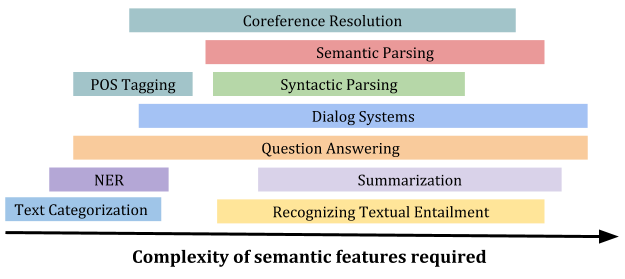
\includegraphics[width=5in]{figures/NLU_spectrum.png} \caption{Various
%NLP tasks organized in terms of the complexity of semantics needed to solve
%them.}\label{fig:nlu_spectrum} \end{center} \end{figure}

\subsection{Parts of an NLU system} Now that we have characterized the tasks we are interested in,
let us identify what goes into building systems for those tasks.  Consider Question Answering (QA),
which refers to answering questions about a span of text, or other structured knowledge
representations like knowledge bases or even images.  QA systems are required to encode the meaning
of the provided inputs such that the relevant bits of information can be retrieved to answer
questions.  Recognizing Textual Entailment (RTE), another NLU task, refers to the problem of
identifying whether the truth value of some text provided as a hypothesis follows from that of
another text provided as a premise, and it is usually done by extracting relevant features from the
hypothesis and the premise to see if there is enough overlap between them in the right direction.
Similarly, Sentiment Analysis requires automatically categorizing the opinions expressed in the
input utterances towards specific targets. This involves extracting appropriate affective states and
subjective information, such that a sentiment classifier can be built using that information as
features. To perform well at at each of these tasks, the NLU systems should encode the semantics of
the input to support the kind of reasoning appropriate for the task.

In each of the examples above, it can be noticed that there are two common steps: \textbf{encoding}
and \textbf{reasoning}. The encoder extracts task-relevant features from the input, and the
reasoning module performs the appropriate computation on top of the features given by the encoder to
produce the desired result. Given this insight, let us attempt to describe a generic NLU system
using the following two equations: \begin{align} \mathbf{e} &= \mathtt{encode}(\mathbf{I})
\label{eq:generic_encoding}\\ \mathbf{o} &= \mathtt{reason}(\mathbf{e}) \label{eq:generic_reasoning}
\end{align} where $\mathbf{I}$ is the set of textual inputs to the NLU system.  For example,
$\mathbf{I}$  are single sentences in Sentiment Analysis and pairs of sentences in RTE\@.
$\textbf{e}$ are intermediate encoded representations of the inputs (which may or may not be task
specific), and $\mathbf{o}$ are the final task specific predictions. For example, in Sentiment
Analysis or RTE, $\mathbf{o}$ are categorical labels indicating the sentiment or entailment
respectively.

\paragraph{Encoding} In older feature-rich methods for NLU, Equation~\ref{eq:generic_encoding} used
to be a mapping of the inputs to a hand designed feature space, typically containing patterns over
word classes based on part-of-speech \citep{corley2005measuring} or Wordnet synsets
\citep{moldovan2001logic}; shallow linguistic features like dependencies \citep{bos2005recognising};
named entity information \citep{tatu2005semantic}; or other features depending on the task. The
choice of features was left to the discretion of the ML-practitioners designing the NLU systems. In
such systems, the modeling emphasis was more on the reasoning component, and the encoding component
did not involve any learning.  More recent systems \citep[among many
others]{bahdanau:14,weston2014memory,hermann2015teaching,Xiong2016DynamicMN,bowman2016fast,yang:16}
use representation learning or deep learning techniques to also learn the parameters of the
$\mathtt{encode}$ function, and typically this is done jointly with learning the parameters of the
$\mathtt{reason}$ function, to ensure that learned representations are relevant to the task.

\paragraph{Reasoning} This step in an NLU system is the one that produces the final prediction. The
complexity of this step depends on the task at hand.  For example, in tasks like Sentiment Analysis
or RTE, where the output is one of muliple classes, assuming that the encoder does a good job at
extracting the relevant features from input, reasoning involves building a classifier for the output
classes that operates on the features extracted \citep{pang2002thumbs}. However, in the case of
semantic parsing for question answering over a knowledge graph, reasoning requires determining how
parts of the question can be linked to nodes and edges in the knowledge graph, and how they can be
composed to obtain a complete translation of the question into a semantic space defined by the
graph, so that the translation, or a logical form, can be executed against the graph to produce the
answer \citep{Zettlemoyer2005LearningTM}.

\section{Knowledge}\label{sec:intro_external_knowledge} We attempted to describe a generic NLU
system in Equations~\ref{eq:generic_encoding} and~\ref{eq:generic_reasoning}, with the assumption
that the information provide by the utterances $\textbf{I}$ alone is sufficient for encoding their
meaning and reasoning over them. However, this is seldom the case, and the generic formulation we
have so far is missing another key input.  Humans use language as a medium to transfer information.
However, since language is aimed at other humans, we often rely on prior knowledge that we share ---
both about the world, and also about how other humans reason --- and communicate efficiently with
each other without explicitly making references to this shared knowledge. This makes the job of
building NLU systems challenging, since they need to process human utterances more or less in
isolation. The utterances themselves seldom contain all the information needed to comprehend them.
The missing information is either part of the background knowledge about the world humans inherently
possess, or is provided by the surrounding context in which the utterance is spoken or written. NLU
systems thus need to access or infer this knowledge to fully comprehend human language.

In principle, a sophisticated model should be able to infer this knowledge given enough annotated
data. Thus, one might argue that NLU system builders should focus on obtaining more data to train
fully supervised systems. Our counter-argument to that is based on the practicality of building NLU
systems, and is twofold: Firstly, it is often difficult to get sufficient high quality labeled data
for most NLU tasks in practice. Any additional knowledge that can augment the information provided
by the data could help build a better model for the task at hand. Secondly, if knowledge about some
aspects of semantics that need to be modeled can be easily obtained, it is inefficient to not use
it, and build a model from scratch hoping that it would learn that knowledge. The modeling capacity
could instead be used for capturing more nuanced aspects of semantics that the data provide. We will
revisit these counter-arguments later in the thesis as we describe concrete tasks.

Given these considerations, it is valuable to study the kinds of knowledge that NLU generally
requires, with the goal of determining the following:
\begin{enumerate}
	\item What knowledge is required to fill in the gaps in the inputs? 
	\item How can we acquire the missing knowledge? 
	\item How can the additional knowledge be incorporated into NLU systems?
	\item How well does the additional knowledge improve task performance in practice?
\end{enumerate}

Since our ultimate goal is to improve the performance of NLU systems, we take a pragmatic approach
for defining the kinds of knowledge required by NLU systems, and further classify them based on our
means for acquiring them or ways of incorporating them into NLU system.  At a high level, we draw a
distinction between two kinds of knowledge: background and contextual, the former is related to
encoding input utterances, and the latter is related to reasoning over them. We now describe them in
detail.

\subsection{Background Knowledge for Encoding} Background knowledge refers to the domain-specific
information needed by NLU systems to fill in the gaps in human utterances to effectively encode
them. In general domains, this knowledge constitutes real world facts and commonsense knowledge, and
in specialized domains, it might include more esoteric information.

Consider encoding the semantics of the following two sentences:
\begin{itemize}
	\item[] \textit{She ate spaghetti with butter.}
	\item[] \textit{She ate spaghetti with chopsticks.}
\end{itemize}
Any effective NLU system that processes these sentences should encode the
differences between the functions of the phrases \textit{with butter} and
\textit{with chopsticks} in the two sentences, to identify that \textit{butter}
is an accompaniment, and \textit{chopsticks} are instruments. To evaluate this
capability, we can measure the performance of an NLU system at the task of
prepositional-phrase (PP) attachment. Ideally, it should predict that
\textit{with butter} attaches to \textit{spaghetti} in the first sentence, and
\textit{with chopsticks} attaches to \textit{ate}.

A system that does not explicitly have access to this information will at best memorize
co-occurrence patterns in the input words.  Using pre-trained vectors to represent input words
provides additional knowledge to the model in the form of co-occurrence statistics obtained from
large corpora. However, it is unclear whether distributional information at the word level alone can
generally substitute for the kind of knowledge described above. Fortunately, for knowledge like
this, one can leverage the information a lexical ontology like WordNet \citep{miller1995wordnet}
gives. For example, WordNet specifies that \textit{butter} is a \textit{diary product}, and
\textit{chopsticks} are \textit{tableware}.

However, not all background knowledge can be explicitly stated. A large portion of what we call
commonsense cannot be expressed in the form of concrete relations like in the example above.  The
following example illustrates the point. Consider the events described by the three sentences:

\begin{itemize} \item[] \textit{Man recovering after being shot by cops.} \item[] \textit{Man
recovering after being bitten by a dog.} \item[] \textit{Man recovering after being shot by a dog.}
\end{itemize}

Clearly, one would find the third sentence more unusual compared to the first and the second, the
reason being that a \emph{dog} performing a \emph{shooting} action does not agree with our knowledge
about the general state of affairs. While this information is not clearly written down anywhere,
humans know it implicitly. An NLU system that is designed to differentiate between these sentences
should be provided with the information that \emph{dog} in the role of the agent for \emph{shooting}
is unlikely, while it can be the patient for \emph{shooting}, and \emph{man} fits equally well as
agent and patient for \emph{shooting}. The challenge then is to automatically acquire this kind of
background knowledge.

Based on these observations, we define two kinds of background knowledge: \textbf{explicit} and
\textbf{implicit} based on their availability in external resources.


\subsection{Contextual Knowledge for Reasoning}
Meaning is often context-dependent. Contexts provide the circumstances under which the meaning of
utterances is finally decoded. Reasoning in those contexts has the pre-requisite of grounding the
inputs in them.  For example, an automated reading comprehension system that is built to answer
questions in some context, after encoding the inputs, is expected to effectively match them against
against some representation of the context provided, to extract the information queried by the
question.  Hence, even after filling in the gaps due to missing background knowledge, an NLU system
may need additional information to link them to (or ground them in) the contexts.  We refer to this
additional information as \textbf{contextual knowledge}.  Like background knowledge, this kind of
knowledge may not be explicitly stated, but unlike background knowledge, this is context-specific and
affects how reasoning can be performed in context.

Depending on the type of contexts over which the given task requires reasoning, different forms of
contextual knowledge may be needed.  In this thesis, we focus on the case where explicit relations
exist among bits of information in the contexts so that they can be represented as knowledge graphs,
and reasoning over them can be performed as a series of discrete operations, thus making it an instance of
\emph{Semantic Parsing}. Contextual knowledge in our case is required to link parts of the inputs to nodes or
edges in the graph, and to set syntactic and semantic constraints on the logical forms produced by
the semantic parser.

Figure~\ref{fig:wikitables_example} shows a question taken from the \textsc{WikiTableQuestions}
dataset \citep{pasupat2015compositional}, and an associated table from a Wikipedia article, which
provides the necessary context to answer it. This an example of a QA task where the context is
structured as a table. As it can be seen from the example, answering this question requires linking
\textit{place} in the question to the \textit{Rank} column, \textit{8th} to the cells with
\textit{8} in them, and \textit{total} to a sum operation, and then doing multi-step reasoning over
the table: finding the rows where the value under the \textit{Rank} column is \textit{8}; extracting
the values under the \textit{Total} column from those rows; and calculating their sum.
\begin{figure}
	\begin{center}
		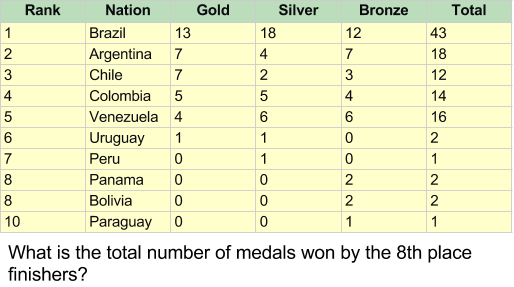
\includegraphics[width=4in]{figures/wikitables_example.png}
	\caption{Example from \textsc{WikiTableQuestions}, a task requiring reasoning over
	structured contexts}\label{fig:wikitables_example}
	\end{center}
\end{figure}

Consider another example of a similar problem in Figure~\ref{fig:nlvr_example_intro}, that requires
evaluating whether the given statement is true or false in the given structured context (the image).
Reasoning in this case involves determining that \textit{box with multiple items} refers to the
presence of muliple objects within one of the three large boxes, \textit{item has different color}
the objects defined by their property \textit{color} being different from the rest of the objects in
the same box, and \textit{one item} refers to the count of such an object being \textit{1}. Further,
reasoning also involves determining the correct order in which these operations need to be
performed. All of this requires contextual knowledge that is not explicitly present in the context.

\begin{figure} \begin{center} 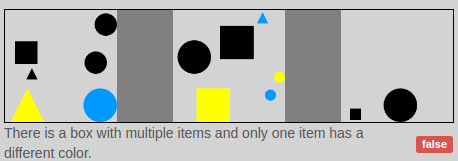
\includegraphics[width=4in]{figures/nlvr_example.png} \caption{Example
from Cornell Natural Language Visual Reasoning (NLVR), a task providing supervision in the form of
binary labels}\label{fig:nlvr_example_intro} \end{center} \end{figure}

In this thesis, we focus on tasks where clear structure exists in contexts. In cases where the
contexts are
unstructured~\citep{hill2015goldilocks,richardson2013mctest,penas2013qa4mre,breck2001looking},
reasoning is not as explicit as was shown in the examples above. Accordingly, the kinds of
contextual knowledge required for those tasks cannot be explicitly stated.  While there are
interesting challenges in solving those tasks, and automatically acquiring the contextual knowledge
required for them, they are beyond the scope of this thesis.

\section{Knowledge-Aware NLU} Given that knowledge, both background and contextual, plays an
important role in several real-world language understanding tasks, we need to reconsider our
definition of the generic NLU pipeline.  Without background knowledge, the encoding of inputs will
be incomplete, and the NLU systems might not generalize beyond the specific patterns seen in the
training data to unseen test cases. Without contextual knowledge, and an effective method to link
encoded inputs to contexts, the NLU systems will simply not have sufficient information to produce
the desired results. We thus modify our NLU equations as follows.  \begin{align} \mathbf{e} &=
\mathtt{encode\_with\_background}(\mathbf{I}, \mathbf{K}_e) \label{eq:encoding_with_knowledge}\\
\mathbf{o} &= \mathtt{reason\_in\_context}(\mathbf{e}, \mathbf{K}_r)
\label{eq:reasoning_with_knowledge} \end{align} where $\mathbf{K}_e$ and $\mathbf{K}_r$ represent
the knowledge required for encoding and reasoning respectively. They come from different sources and
augment the NLU systems in different ways.

\subsection{Better encoding with background knowledge} $\mathbf{K}_e$ is additional knowledge used
to fill in the semantic gaps in the inputs, and thus obtain better encoded representations of them.
One source of such background knowledge is knowledge bases and ontologies, which encode it
explicitly. Examples include hypernym trees from WordNet for incorporating sense and generalization
information about concepts while composing sentences and subgraph features from Freebase to encode
relations between entities seen in the input text.~\cite{moldovan2001logic}
and~\cite{krymolowski1998incorporating} are examples of a feature-rich systems that encoded input
sentences in the context of external knowledge. Both systems used WordNet features and other related
information about the semantic classes of the words in the input in NLU tasks.
While~\cite{krymolowski1998incorporating} built a system based on SNoW \citep{CCRR99} for predicting
Prepositional Phrase Attachment,~\cite{moldovan2001logic} built a QA system. In
Chapter~\ref{chapter:ontolstm} we describe a representation-learning application of knowledge-aware
encoding where we show the advantages of incorporating WordNet information in recurrent neural
networks for encoding sentences.

Adding external knowledge inputs to NLU systems is not straightforward. Firstly, while linking text
being read to some structured background knowledge in a KB, an automated system usually faces
considerable ambiguity. For example, with lexical ontologies like WordNet, we get useful type
hierarchies like \textit{parent is-a ancestor is-a person} and \textit{pool is-a body-of-water} and
so on, but one has to deal with sense ambiguity: \textit{pool} can also be a game. Another challenge
stems from the fact that most KBs represent meaning in a symbolic fasion, whereas most modern NLU
systems are based on neural network models, and represent textual inputs in a continuous space.
Chapter~\ref{chapter:ontolstm} focuses on learning distributions over the discrete concepts of the
KB conditioned on the context, to deal with exceptions in language.

Explicit sources of knowledge are often incomplete, or may not contain the kind of knowledge needed
to fill the gaps to obtain representations need for the task at hand.  An alternative source of
background knowledge is the co-occurrence of slot-fillers, given an appropriate structured
representation of the inputs: Assuming we have correctly identified the structure within the inputs,
we can leverage large corpora to obtain expected semantics of the fillers of the roles of defined by
the structure, and use those expectations to judge the given inputs.  This idea is very similar to
Selectional Preference, the notion that a verb places semantic restrictions on the subjects and
objects it can take \citep{katz1963structure,wilks1975preferential}.  This notion was successfully
used in modeling semantics within syntactic structures for sense disambiguation
\citep{resnik1997selectional} and metaphor identification \citep{shutova2013statistical}, among
others.  In Chapter~\ref{chapter:nem}, we take this idea further to model selectional preferences
within predicate argument structures, to learn representations of of the implicit knowledge required
to distinguish anomalous newswire events from normal ones.

\subsection{Reasoning with contextual knowledge} $\textbf{K}_r$ inputs allow NLU systems reason
using additional contextual knowledge. Within this thesis, we focus on those tasks where reasoning
can be viewed as semantic parsing problems.  The contexts are often structured in this case. There
exist both traditional \citep[among
others]{Zelle1996LearningTP,Zettlemoyer2005LearningTM,zettlemoyer2007online} and neural network
based methods
\citep{Dong2016LanguageTL,Andreas2016LearningTC,Liang2016NeuralSM,Neelakantan2016LearningAN} for
solving these problems. 

Depending on the level of supervision provided, training semantic parsers might require additional
contextual knowledge. If logical form supervision is not available
\citep{berant2013semantic,pasupat2015compositional,krishnamurthy2017neural}, semantic parsing
involves some form of a search over the logical form space to find those that correspond to the
sequence of operations that result in the correct answer.  In that case, contextual knowledge about
the restrictions of the logical form space can be used to constrain the search process,
\citep{xiao2016sequence,krishnamurthy2017neural}, thus making reasoning more efficient.

In the example shown in Figure~\ref{fig:wikitables_example}, the supervision comes only from the
answers. This can be used to drive the search process, since the requirement that the resulting
logical form should evaluate to the given answer restricts the search space to a large extent.
Figure~\ref{fig:nlvr_example_intro} also shows an example where the supervision comes only from the
answers. However, since the answers are binary, they do not restrict the search space as much. In
fact, given a space of valid logical forms, exactly 50\% of them evaluate to the given answer, but
only a minute proportion of them are true translations of the given sentence. In this case, when
supervison provided is weaker, we have to rely more on contextual knowledge to ensure that the
produced logical form involves reasoning relevant to the input sentence.

In this thesis, we first describe a type driven neural semantic parsing framework in
Chapter~\ref{chapter:wikitables}, where we define a concrete grammar over the space of logical
forms, and use the constraints from the grammar to drive the search process. We also define an
entity linking mechanism trained joinly with the parser to allow the parser to reason about
previously unseen entities. Then, in Chapter~\ref{chapter:nlvr}, we deal with the issue of weaker
supervision from binary labels. The contextual knowledge in this case is a compositional logical
form language we define, where the functions are easily mappable to natural language utterances. We
exploit the properties of this language to propose a lexicon-guided coverage mechanism that drives
the search process towards logical forms that use operations relevant to input utterances.  We show
that this technique is necessary for domains with binary denotations. Additionally, we present an
iterative search method, that alternates between searching for programs that give correct answers,
and maximizing the likelihood of retrieved ones, thereby exploiting the compositionality of the
target language to produce increasingly complex programs. 

\subsection{Evaluating NLU Performance} The effectiveness of NLU systems is often measured in terms
of their performance at the intended task. The inherent assumption behind taking a task-oriented
approach towards building NLU systems is that an improvement in the task performance correlates with
an improvement in the quality of the semantic representation, and the understanding capability of
the computational system.  We design our evaluation pipelines in this thesis based on this
assumption.

For example, in Chapter~\ref{chapter:ontolstm}, where we incorporate background knowledge from
WordNet into sentence level encoders, we evaluate the effect of the proposed improvement by
measuring the task performance with and without the knowledge incorporated from WordNet. Similarly,
in Chapter~\ref{chapter:nem}, we argue that encoding selectional preferences results in better event
representations, and we evaluate that claim by comparing the performance of a model that encodes
selectional preferences with that of another that does not, at the task of predicting
newswire event anomalies.

We test the quality of the encoded representations by running controlled experiments that measure
task performance. While interpreting the encoded representations is also an active research
topic, it is beyond the scope of this thesis.

\section{Thesis Contributions and Outline}
In this thesis, we make the following claims, and provide empirical evidence for them:
\begin{enumerate}
	\item While encoding utterances, incorporating relevant symbolic background knowledge results
		in better representations of inputs.
	\item When relevant background knowledge is not explicitly stated in symbolic form,
		it can be induced by modeling selectional preferences within appropriate predicate argument
		structures extracted from the input utterances.
	\item For reasoning tasks that can be cast as problems involving search over a space of
		discrete compositional operations, incorporating knowledge about the syntax and semantics
		of the operations into the search process results in more effective reasoning modules.
	\item Furthermore, knowledge about the compositionality of the target operator space
		can be exploited to define a training procedure that can effectively deal with the
		problem of spuriousness, a significant challenge when training models with weak
		supervision.
\end{enumerate}

The document is organized as follows:

Chapter~\ref{chapter:encoding_related_work} describes the previous work done in encoding utterances
at various levels of granularity, and the attempts to incorporate background knowledge into
the learned representations.

In Chapter~\ref{chapter:ontolstm}, we describe a method to incorporate explicit knowledge from
WordNet towards obtaining better sentence representations. Our model looks at WordNet synsets and at
the hypernym hierarchies of the words being processed, making the encoder aware of their different
senses and the corresponding type information. Concretely, we transform a popular variant of
recurrent neural-network model, one with Long Short-Term Memory (LSTM) \citep{hochreiter1997long},
to incorporate ontological information.  The ontology-aware LSTM (OntoLSTM) learns to attend to the
appropriate sense, and the relevant type (either the most specific concept or a generalization by
choosing a hypernym of the word), conditioned on the context and the end-objective. We show that the
sentence representationsproduced by OntoLSTM are better than those produced by LSTMs when used with
identical prediction components for predicting textual entailment and preposition phrase attachment.
We also visualize the attention scores assigned to the hypernyms of words in the input sentences and
show that OntoLSTM is indeed learning useful generalizations of words that help the learned
representations perform better at the end task.

In Chapter~\ref{chapter:nem} we encode events as predicate argument structures derived from a
semantic role labeler.  In this chapter, we rely on selectional preferences between verbs and their
semantic role fillers as the background knowledge, and show how they are useful in predicting
anomalous events.  Our event encoder, Neural Event Model (NEM) captures semantics deeper than the
surface-level fluency. We describe an annotation effort that resulted in newswire headlines manually
labeled with the degree of surprise associated with them and show that NEM outperforms a baseline
LSTM model that encodes sentences at anomaly detection. 

Chapter~\ref{chapter:reasoning_related_work} provides context for reasoning over grounded language
with discrete operations, and various training methods used for dealing with the issue of weak
supervision when the reaoning problem is viewed as learning semantic parsers from question-answer
pairs.

Chapter~\ref{chapter:wikitables} deals with reasoning over tables as structured contexts. We
describe a type-driven neural semantic parser aimed at answering compositional questions about
Wikipedia tables. It is an encoder-decoder model that generates well-typed logical forms that can be
executed against graph representations of the tables in context. The parser also includes entity
embedding and linking modules that are trained jointly using QA supervision. We show results on 
the \textsc{WikiTableQuestions} dataset.

In Chapter~\ref{chapter:nlvr}, we describe the lexicon-coverage guided search process to deal with
lack of sufficient supervision in domains with binary labels like Cornell NLVR\@.  The chapter also
includes an iterative search and maximization algorithm where we exploit the compositionality of the
logical form language to produce increasingly complex logical forms. We show that this technique is
generally applicable to training semantic parsers with weak supervision, and show state of the art
results on NLVR and \textsc{WikiTableQuestions}.

Finally, in Chapter~\ref{chapter:conclusion}, we describe several potential directions for
future research, building on top of the tasks we studied in this thesis, and the kinds of knowledge
we exploited. As a concrete example, we discuss how the techniques presented in
Chapters~\ref{chapter:wikitables} and~\ref{chapter:nlvr} can be extended to unstructured contexts,
and the challenges that come with doing so, as a motivation for future work in this area.
